\documentclass[11pt,a4paper]{article}
\usepackage[utf8]{inputenc}
\usepackage[T1]{fontenc}
\usepackage{amsmath,amssymb,amsthm}
\usepackage{graphicx}
\usepackage[margin=2.5cm]{geometry}
\usepackage{hyperref}
\usepackage{xcolor}
\usepackage{booktabs}
\usepackage{authblk}
\usepackage{cite}
\hypersetup{colorlinks=true,linkcolor=blue,citecolor=blue,urlcolor=blue}

\title{\textbf{Discrete Drainage Dynamics VII:\\
Gravity--Gauge Coupling and the Joint Wilson-Loop\\
Back-Reaction}}
\author[1]{Stanislas Dewavrin}
\affil[1]{Independent researcher \\ \texttt{dewavrin.iphone@gmail.com}}
\date{May 2026}

\begin{document}
\maketitle

\begin{abstract}
\noindent
Paper~II derives gravity from the back-reaction of scalar
drainage on the substrate, with mobility $\mu(R)$. Paper~VI
derives a candidate fixed-point formula for $\alpha_{\rm EM}$
from the back-reaction of a Wilson loop along the body diagonal
of the unit cube. Both mechanisms share the same physical
substrate; the present paper examines what their coupling
implies. We argue that on the unit cube, two distinct
back-reaction loops coexist---the body-diagonal Wilson loop
(length $\sqrt{3}$) carrying $\alpha_{\rm EM}$, and the
cube-surface Wilson surface (area $6$) carrying the
gravitational coupling at the substrate scale. Under the
assumption that the two sectors share the same combinatorial
prefactor and one-loop structure, we obtain a leading
\emph{tree-level structural} ratio
$\alpha_G^{\rm lat}/\alpha_{\rm EM}^{\rm lat}
= \sqrt{3/6} = 1/\sqrt{2}$. Anchoring this ratio with the
laboratory low-energy value $\alpha_{\rm EM}(0) = 1/137.036$
yields a phenomenological substrate mass scale $m_{\rm lat}
\approx 0.072\,M_P$ and lattice spacing $\ell_{\rm lat}
\approx 14\,\ell_P$ (a full running-coupling treatment is
deferred). Under a minimal local-reserve coupling ansatz
$\varepsilon_{\rm local}(R) = \varepsilon_0 R/R_0$, two
cross-coupling effects follow: a gravitational modulation of
$\alpha_{\rm EM}$ proportional to $|\Phi_{\rm grav}|/c^2$ near
massive bodies, and an EM-induced drainage proportional to the
local Maxwell stress-energy. Cosmological drift of $\alpha_{\rm
EM}$ inherited from a slowly-varying $R_0$ is potentially in
tension with current atomic-clock bounds for an $O(1)$ Hubble
fraction, providing the most stringent immediate falsifier. This
construction reframes the apparent weakness of gravity as a
\emph{scale hierarchy}: at the substrate scale the two
couplings are geometrically comparable, while ordinary particles
lie far below that scale. The paper proposes a structural
closure between Papers~II and~VI: one substrate, one
back-reaction principle, two emergent couplings sharing a
common geometric origin.
\end{abstract}

\noindent\fbox{\parbox{0.96\textwidth}{\small
\textbf{What this paper makes mechanically legible.}
GR and SM provide gravity ($G$) and electromagnetism ($\alpha_{\rm EM}$) as independent empirical inputs --- there is no first-principles relation between them in the standard formalism, and the hierarchy $\alpha_G/\alpha_{\rm EM}$ is treated as accidental. \emph{This paper} observes that the same discrete substrate hosts two distinct back-reaction loops on the unit cube: the body-diagonal Wilson loop (length $\sqrt{3}$) carrying $\alpha_{\rm EM}$ (Paper~VI), and the cube-surface Wilson surface (area $6$) carrying gravity (extension of Paper~II). Under the labelled hypothesis (H-shared-prefactor), the leading tree-level structural ratio is $\alpha_G^{\rm lat}/\alpha_{\rm EM}^{\rm lat} = \sqrt{3/6} = 1/\sqrt{2}$. \textbf{Leverage:} the gravity-gauge ratio is converted from accidental empirical input into a candidate combinatorial quantity of the substrate's unit cube; anchoring with CODATA $\alpha_{\rm EM}(0)$ then yields phenomenological $m_{\rm lat} \approx 0.072\,M_P$ and $\ell_{\rm lat} \approx 14\,\ell_P$, both falsifiable.
}}
\bigskip


\paragraph{Programme positioning and analogue framing.}
DDD does not contest GR or the SM; gravity at observable distances and the empirical $\alpha_{\rm EM}$ are anchors. The novelty of this paper is the assertion of a \emph{relation} between two quantities the standard formalism treats as independent. The result is internal to the analogue and conditional on (H-shared-prefactor); GR/SM remain valid in their respective domains.


\paragraph{Which mystery does this paper address?}
Per SERIES\_FEEDBACK §0.bis, this paper targets:

\begin{itemize}
\item \textbf{Mystery~\#3 (fine-structure) + \#2 (gravitational coupling) jointly.} SM/GR provide $\alpha_{\rm EM}$ and $G$ as independent inputs. This paper proposes a structural ratio between them based on the body-diagonal vs cube-surface combinatorics on the unit cube. The form $\sqrt{3/6}$ is a substrate consequence of the labelled hypothesis (H-shared-prefactor); the value of $\alpha_{\rm EM}$ remains calibrated against CODATA, but the ratio is structurally predicted.
\end{itemize}


\paragraph{Distinctive contribution and ontological reading.}
SM/GR has no structural relation between $\alpha_G$ and $\alpha_{\rm EM}$; their independence is just an empirical fact. This paper's distinctive contribution is a \emph{combinatorial relation}: on the unit cube, two natural Wilson objects (body diagonal length $\sqrt{3}$ and cube surface area $6$) host the EM and gravitational back-reactions respectively, and under (H-shared-prefactor) their lattice couplings stand in the ratio $\sqrt{3/6} = 1/\sqrt{2}$. The leverage: (a) the gravity-gauge hierarchy is partially derived from substrate geometry; (b) the resulting phenomenological scales ($m_{\rm lat} \approx 0.072\,M_P$, $\ell_{\rm lat} \approx 14\,\ell_P$) are concrete and testable; (c) cross-coupling effects (gravitational modulation of EM, EM modulation of gravity) become structurally predicted, where SM/GR cannot speak.


\section{Main claims and scope}
\label{sec:claims}

\begin{enumerate}
\item \textbf{One substrate, two back-reaction loops.}
The gravitational and electromagnetic sectors of DDD share the
same cubic substrate. On the unit cube, two distinct closed
Wilson objects coexist: the body diagonal (a $1$D loop of
squared length $3$) carrying the U(1) gauge phase of Paper~VI,
and the cube surface (a $2$D Wilson surface of area $6$)
carrying the gravitational drainage of Paper~II. They are
\emph{not} the same loop, and they back-react on different
geometric quantities.

\item \textbf{Tree-level structural ratio at the substrate
scale.}
Under the assumption that the two sectors share the same
combinatorial prefactor $8\pi^2 = 4\,\mathrm{Vol}(S^3)$ and the
same one-loop structure but with different characteristic
lengths, the leading structural ratio is
\begin{equation}
\boxed{\;
\frac{\alpha_G^{\rm lat}}{\alpha_{\rm EM}^{\rm lat}}
\;=\; \sqrt{\frac{x_{\rm EM}}{x_{\rm grav}}}
\;=\; \sqrt{\frac{3}{6}}
\;=\; \frac{1}{\sqrt{2}}.
\;}
\label{eq:grav-em-ratio-VII}
\end{equation}
This is a leading structural prediction conditional on the
shared Wilson-loop prefactor; it is not yet verified at one loop
in the joint sector (\S\ref{sec:joint-WL}).

\item \textbf{Phenomenological substrate mass scale at $\sim
0.072\,M_P$.}
Combining \eqref{eq:grav-em-ratio-VII} with the
laboratory low-energy value $\alpha_{\rm EM}(0) = 1/137.036$
(used here as a phenomenological anchor; a full running-coupling
treatment between the substrate scale and laboratory scale is
deferred) and the defining relation $\alpha_G(m) = (m/M_P)^2$
gives
\begin{equation}
\frac{m_{\rm lat}}{M_P} \;=\; \sqrt{\frac{1}{137.036\,\sqrt{2}}}
\;\approx\; 0.072,
\end{equation}
which fixes the substrate's characteristic mass at $\sim
0.072\,M_P \approx 8.8 \times 10^{17}\,\text{GeV}$ and the
lattice length scale at $\ell_{\rm lat} \approx 14\,\ell_P$.

\item \textbf{Two cross-coupling consequences from a minimal
ansatz.}
Under the minimal local-reserve coupling ansatz
$\varepsilon_{\rm local}(R) = \varepsilon_0\,R/R_0$, the shared
substrate generates two leading-order cross-coupling effects:

\textit{(i) Gravity modulates $\alpha_{\rm EM}$:} the body-diagonal
Wilson loop near a mass $M$ sees a depleted reserve $R(r)/R_0
= \sqrt{1 - \beta/r}$ (Paper~II), shifting the effective
$x_{\rm EM}^*$ and hence $\alpha_{\rm EM}$ by an amount of
order $\delta\alpha/\alpha \sim |\Phi_{\rm grav}|/c^2$ at
distance $r$ from the source.

\textit{(ii) EM modulates $G$:} the local Maxwell stress-energy
contributes to substrate drainage just as ordinary mass-energy
does, generating a small additional gravitational potential
proportional to $\rho_{\rm EM} = (E^2 + B^2)/(8\pi)$.
\end{enumerate}

\textbf{Limitations and scope.}
We do not derive the absolute value of Newton's $G$ in SI
units; that is the calibration result of Paper~II.
We do not compute Standard Model fermion masses; their hierarchy
relative to $m_{\rm lat}$ is the subject of Paper~XV.
We do not address how strong or weak nuclear interactions emerge.
The cross-coupling magnitudes derived below are leading-order
estimates based on the back-reaction structure inherited from
Papers~II and~VI; precision predictions require analytical
closure of the open problems listed in those papers (the
small-world correction $\varepsilon$ and the exact one-loop
coefficient $V_{d_{\rm eff}}$).

\subsection*{Motivation and significance}
\addcontentsline{toc}{subsection}{Motivation and significance}

One of the long-standing puzzles of fundamental physics is the
enormous apparent weakness of gravity compared with
electromagnetism at ordinary particle scales. For two electrons,
the gravitational coupling is smaller than the electromagnetic
one by roughly forty orders of magnitude. In standard units this
hierarchy is usually expressed through the small ratio
$m_e/M_P$, but the question remains: why should gravity be so
weak for the particles we observe?

The present paper proposes a DDD interpretation of this
hierarchy. Gravity and electromagnetism are not treated as
unrelated mechanisms. They are two back-reaction channels of the
same discrete substrate, associated with two distinct closed
objects on the unit cube: a body-diagonal Wilson loop for the
gauge sector and a cube-surface Wilson surface for scalar
drainage. At the substrate scale, their leading structural ratio
is not exponentially small but geometric,
\begin{equation*}
\frac{\alpha_G^{\rm lat}}{\alpha_{\rm EM}^{\rm lat}}
\;=\; \frac{1}{\sqrt{2}},
\end{equation*}
conditional on the shared Wilson-loop prefactor.

In this reading, gravity is not intrinsically weak at the
substrate scale. It appears weak at laboratory scales because
ordinary particle masses lie far below the substrate mass scale.
Anchoring the structural ratio with the low-energy value of
$\alpha_{\rm EM}$ gives a phenomenological substrate scale
$m_{\rm lat}\sim 0.07\,M_P$, and the smallness of gravitational
effects for electrons is shifted into the mass hierarchy
$m_e/m_{\rm lat}$.

This paper therefore does not claim a complete unification of
forces. It proposes a more limited \emph{structural bridge}: one
substrate, one back-reaction principle, and two emergent
couplings associated with different closed geometric objects.
The remaining tasks are explicit: compute the joint one-loop
correction, derive the local reserve-dependence of the effective
dimension, and (in Paper~XV) explain the hierarchy between
Standard Model masses and $m_{\rm lat}$.

The same bridge produces falsifiable consequences. If the local
reserve modifies the effective small-world dimension, then
massive bodies should induce a small modulation of $\alpha_{\rm
EM}$, and cosmological evolution of the reference reserve $R_0$
should induce a secular drift of $\alpha_{\rm EM}$. The
hierarchy puzzle, the gravity--gauge relation, and possible
variation of fundamental constants thus become linked to the
same substrate coupling and become testable on a common
experimental front. Figure~\ref{fig:scale-hierarchy} summarises
the scale picture.

\begin{figure}[h]
\centering
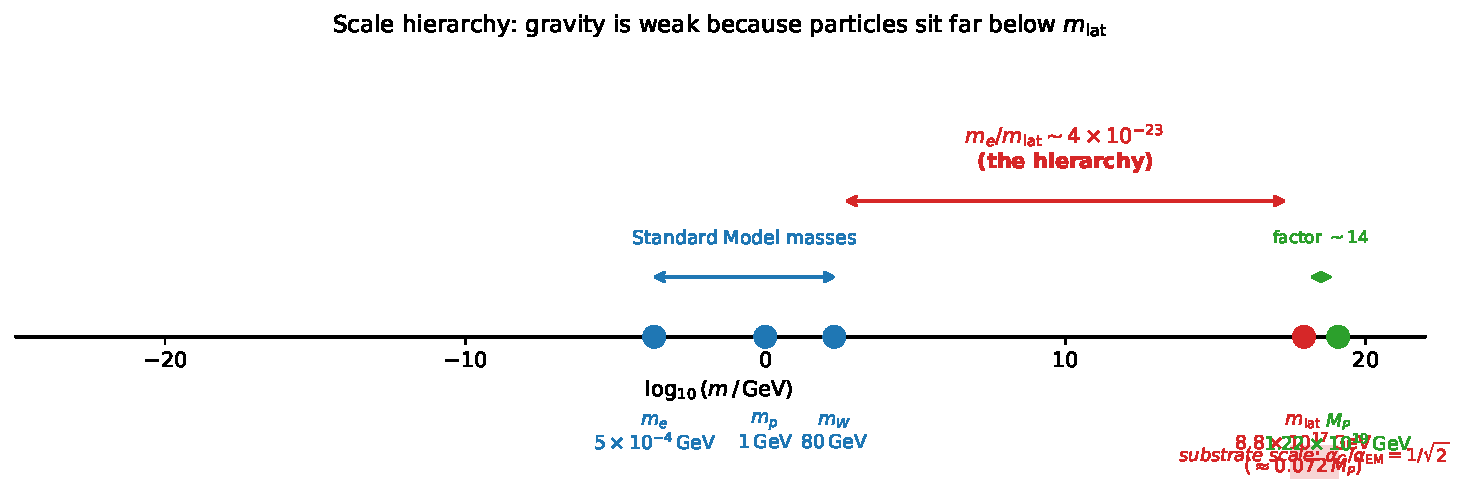
\includegraphics[width=0.98\textwidth]{figures/fig5_scale_hierarchy.pdf}
\caption{Scale hierarchy interpretation. Standard Model masses
sit at $\sim 10^{-3}$ to $10^2$~GeV, $\sim 23$ orders of
magnitude below the substrate mass scale $m_{\rm lat} \approx
0.072\,M_P \approx 8.8 \times 10^{17}$~GeV. The substrate is
itself a factor $\sim 14$ below the Planck mass. At the
substrate scale, gravity and electromagnetism are comparable
($\alpha_G/\alpha_{\rm EM} = 1/\sqrt{2}$); the observed
weakness of gravity for ordinary particles is a consequence of
the ratio $m_e/m_{\rm lat} \sim 4 \times 10^{-23}$, not of any
fundamental weakness of the gravitational coupling.}
\label{fig:scale-hierarchy}
\end{figure}

\section{Physical picture in plain words}
\label{sec:picture}

\textbf{The mystery.} Gravity looks absurdly weak compared with
electromagnetism at ordinary scales. Two electrons repel
electrically far more strongly than they attract gravitationally
--- by roughly forty orders of magnitude. In DDD, Paper~VII
suggests that this weakness may not be fundamental. At the
substrate scale, gravity and electromagnetism may be two nearly
comparable back-reactions of the same discrete medium. The
enormous hierarchy appears only when one asks how a very light
particle, such as the electron, samples that substrate.

Imagine the substrate of the previous papers as a vast
3-dimensional jungle gym of nodes and links. Paper~II said: at
each node lives a reserve of energy that can drain locally, and
when a mass concentrates somewhere, the drainage rate is
modified, which back-reacts on the local clock-rate.
That gives gravity. Paper~VI said: each link also carries a
phase, and when you trace the smallest closed body-diagonal
loop, the resulting Wilson loop self-energy fixes the strength
of the electromagnetic coupling. That gives $\alpha_{\rm EM}$.

\textbf{The natural question.} If both stories live on the
same substrate, do they interact? The answer, in DDD, is yes,
and the interaction is geometric, not added by hand.

\textbf{Two loops on one cube.} The body diagonal of the unit
cube has squared length $3$. The boundary of the cube (its six
faces) has total area $6$. These are the two simplest closed
objects you can build out of one cube of substrate. The
body-diagonal loop carries the gauge sector and gives
$\alpha_{\rm EM}$. The cube-surface object carries the drainage
flux through the cube's faces and gives the gravitational
coupling at the substrate scale, $\alpha_G^{\rm lat}$. Same
prefactor (it comes from the same combinatorial multiplication
$4 \times \mathrm{Vol}(S^3) = 8\pi^2$), but a different
characteristic length squared. So:
\begin{equation*}
\alpha_{\rm EM}^{\rm lat} \;=\; \frac{1}{8\pi^2\sqrt{3}},
\qquad
\alpha_G^{\rm lat} \;=\; \frac{1}{8\pi^2\sqrt{6}},
\qquad
\frac{\alpha_G^{\rm lat}}{\alpha_{\rm EM}^{\rm lat}}
\;=\; \frac{1}{\sqrt{2}}.
\end{equation*}

\textbf{What scale is this?} A coupling of order $5 \times
10^{-3}$ for gravity is enormous compared to its everyday value
(electron-to-electron gravity has $\alpha_G \sim 10^{-45}$). But
the everyday value is evaluated for particles whose masses are
tiny compared with the substrate scale. At the substrate,
gravity and electromagnetism are within a factor $\sqrt{2}$ of
each other. \emph{The hierarchy is therefore not placed in the
relative strength of the two substrate couplings, but in the
ratio between observed particle masses and $m_{\rm lat}$.}
Anchoring against the laboratory $\alpha_{\rm EM}(0)$ places the
substrate at $m_{\rm lat} \approx 0.07\,M_P$, about $14$ Planck
lengths in linear extent (subject to a future running-coupling
refinement).

\textbf{Cross-coupling.} Because the two back-reactions live on
the same substrate, each can modulate the other---once we fix
how the local reserve $R$ enters the small-world correction
$\varepsilon$. Under the simplest linear ansatz, a nearby mass
depletes $R$, which shifts the body-diagonal loop's effective
length, which shifts $\alpha_{\rm EM}$. An electromagnetic field
carries energy, which contributes to drainage, which shifts the
gravitational potential. Both effects are calculable in
principle; both are below current sensitivity at laboratory
potentials but the cosmological version is already in the
window of atomic-clock bounds.

\section{Setup: the two sectors on a shared substrate}
\label{sec:setup}

\subsection{The gravitational sector (recap of Paper~II)}

Each node $i$ carries a non-negative scalar reserve $R_i \geq
0$. The local update rule is gradient-descent of a drainage
functional with mobility $\mu(R)$; in the presence of a
mass-energy distribution $\rho(\mathbf{x})$, the steady-state
solution gives the radial profile
\begin{equation}
R^2(r)/R_0^2 \;=\; 1 - \frac{\beta}{r},
\qquad \beta = 2GM/c^2,
\label{eq:Schwarzschild-DDD}
\end{equation}
which is the Schwarzschild $g_{00}$ component of GR (Paper~II,
\S5--7).

\subsection{The gauge sector (recap of Paper~VI)}

Each node carries an additional orientation phase $\alpha_i \in
[0, 2\pi)$, each link carries a U(1) gauge phase $\psi_{ij} \in
[0, 2\pi)$, and the local energy
\begin{equation}
E_{\rm orient} = \sum_{(i,j)} J_{ij}\,
\big[1 - \cos(\alpha_j - \alpha_i + \psi_{ij})\big]
\label{eq:Eorient-VII}
\end{equation}
gives compact U(1) lattice gauge dynamics. The body-diagonal
Wilson loop self-energy yields
\begin{equation}
\alpha_{\rm EM}^* \;=\; \frac{1}{8\pi^2 \sqrt{x_*}},
\qquad x_* = 3 + \alpha_{\rm EM}\sqrt{3}\,
(1 - \alpha_{\rm EM} V_{d_{\rm eff}}),
\label{eq:alpha-EM-recap}
\end{equation}
matching CODATA at sub-ppm level for $d_{\rm eff} = 3 +
\varepsilon$ with $\varepsilon \in \{1/(3\pi),\,1/(2\pi),\,
1/6\}$ (Paper~VI, \S5).

\subsection{The shared substrate}

The same nodes carry both $R_i$ and $\alpha_i$; the same links
carry both the link-state of Paper~III and the gauge phase
$\psi_{ij}$. The combined energy is
\begin{equation}
E_{\rm tot} \;=\; E_{\rm reserve}[R] + E_{\rm orient}
[\alpha, \psi],
\label{eq:E-tot}
\end{equation}
and the dynamics is gradient descent of \eqref{eq:E-tot} with
the appropriate mobility for each sector. Cross-coupling arises
because the local substrate state $R_i$ enters $\mu_{ij}$, the
mobility of the link, which can in principle depend on the
neighbouring orientation phases as well. We do not specify the
exact form of $\mu(R, \alpha, \psi)$ here; we examine the
leading consequences of the simplest natural coupling.

\section{Joint Wilson-loop back-reaction}
\label{sec:joint-WL}

\subsection{Two distinct closed objects on the unit cube}

The unit cube admits two natural closed Wilson objects:

\textbf{Body-diagonal loop.} The body diagonal connects opposite
corners through the cube's interior, with squared Euclidean
length $3$. There are four such diagonals per cube. This is
the elementary Wilson \emph{loop} of the gauge sector. Closure
along this loop provides the perimeter for the
$\alpha_{\rm EM}$ self-consistency.

\textbf{Cube surface.} The boundary of the cube comprises six
square faces, total area $6$. There are four cubes sharing any
given node. The cube surface is the elementary Wilson
\emph{surface} of the scalar sector: drainage flux out of
the cube must close. Surface area $6$ provides the
``perimeter'' for the gravitational self-consistency.

These two objects are geometrically distinct but share the same
substrate combinatorics, namely the four body-diagonal lines
and the spinor $S^3$ phase space (Paper~III). Figure~\ref{fig:two-wilson} illustrates the two
elementary closed Wilson objects.
The shared combinatorial prefactor is
\begin{equation}
N_{\rm geom} \;=\; 4 \times \mathrm{Vol}(S^3)
\;=\; 4 \times 2\pi^2 \;=\; 8\pi^2,
\label{eq:Ngeom}
\end{equation}
identical for both sectors \emph{by hypothesis}; this assumption
is part of what \S\ref{sec:joint-WL}--\ref{sec:m-lat} are
testing.

\begin{figure}[h]
\centering
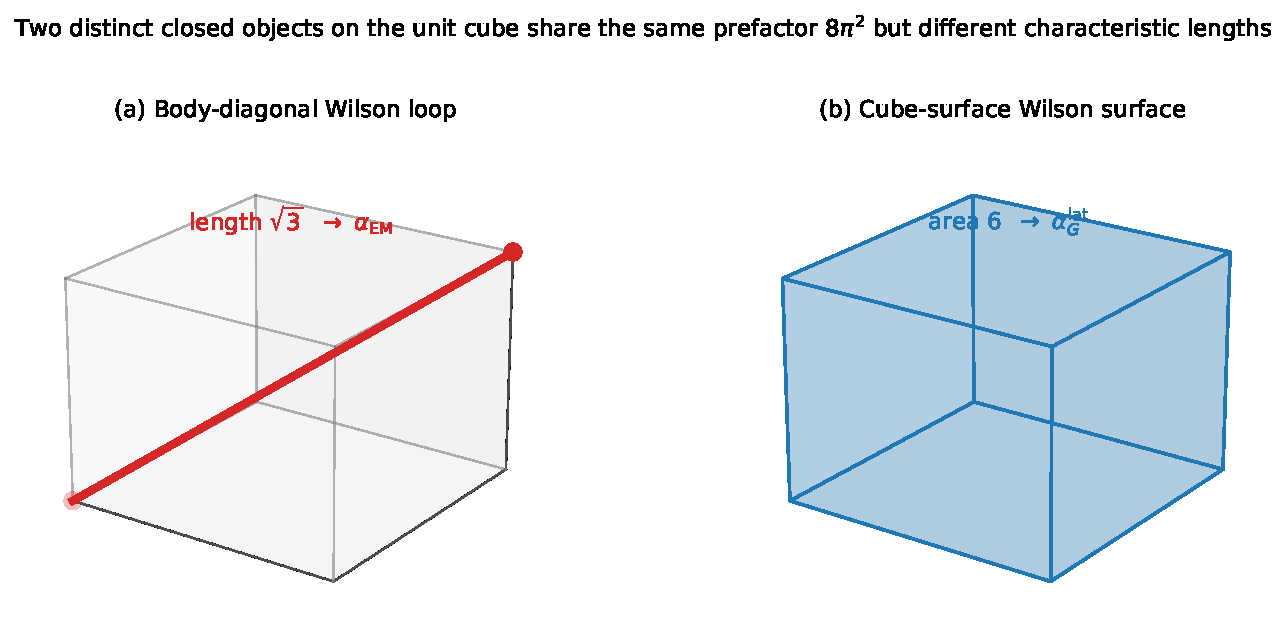
\includegraphics[width=0.95\textwidth]{figures/fig1_two_wilson_objects.pdf}
\caption{The two elementary closed Wilson objects on the unit
cube. \textbf{(a)} The body-diagonal Wilson loop has squared
length $3$ and back-reacts on its own perimeter; this is the EM
self-consistency of Paper~VI. \textbf{(b)} The cube-surface
Wilson surface has total area $6$ and back-reacts on the
gravitational drainage flux; this is the gravitational
analogue. Both share the same combinatorial prefactor
$N_{\rm geom} = 8\pi^2$, leading to the structural ratio
$\alpha_G^{\rm lat}/\alpha_{\rm EM}^{\rm lat} = \sqrt{3/6} =
1/\sqrt{2}$.}
\label{fig:two-wilson}
\end{figure}

\subsection{Coupling structures from the two loops}

For each loop type, we postulate the same back-reaction form
\eqref{eq:alpha-EM-recap}. At lowest order (tree level, before
including the back-reaction):
\begin{align}
\alpha_{\rm EM}^{(0)} &\;=\; \frac{1}{N_{\rm geom}\sqrt{x_{\rm EM}}}
\;=\; \frac{1}{8\pi^2\sqrt{3}}, \\
\alpha_G^{{\rm lat},(0)} &\;=\; \frac{1}{N_{\rm geom}\sqrt{x_{\rm grav}}}
\;=\; \frac{1}{8\pi^2\sqrt{6}}.
\end{align}
The structural ratio is therefore
\begin{equation}
\frac{\alpha_G^{{\rm lat},(0)}}{\alpha_{\rm EM}^{(0)}}
\;=\; \sqrt{\frac{3}{6}} \;=\; \frac{1}{\sqrt{2}},
\label{eq:ratio-tree}
\end{equation}
fixed by geometry alone, conditional on the shared
prefactor. We refer to this as the \emph{tree-level structural
ratio} of the joint sector. Whether this ratio survives at one
loop is conditional on the loop coefficients of the two sectors
matching, which is not yet established.

\subsection{One-loop conditional robustness}

Both sectors receive a small back-reaction correction (one-loop
volume integral, two-loop, etc.). Schematically, at one loop:
\begin{align}
\alpha_{\rm EM} &= \frac{1}{8\pi^2\sqrt{x_{\rm EM}^*}},
& x_{\rm EM}^* &= 3 + \alpha_{\rm EM}\sqrt{3}(1 - \alpha_{\rm EM}V), \\
\alpha_G^{\rm lat} &= \frac{1}{8\pi^2\sqrt{x_{\rm grav}^*}},
& x_{\rm grav}^* &= 6 + \alpha_G^{\rm lat}\sqrt{6}(1 - \alpha_G^{\rm lat}V),
\end{align}
with the same $V = V_{d_{\rm eff}}$ in both. \emph{If} the
one-loop coefficient is shared between the two sectors (a
non-trivial assumption: scalar drainage and U(1) gauge degrees
of freedom may have distinct multiplicities, signs, and
spin-related prefactors), the relative shift $\sim \alpha V \sim
0.03$ is identical and the ratio $\alpha_G/\alpha_{\rm EM}
= \sqrt{3/6}$ is preserved up to corrections of order $\alpha^2
V^2 \sim 10^{-3}$. If the loop coefficients differ by an
$O(1)$ factor between the sectors, the ratio receives a
correction at the same percent level. A direct one-loop
computation in the joint sector is open and is the principal
technical task left for Paper~VII--companion work.

\section{The substrate mass scale}
\label{sec:m-lat}

\subsection{Translation to the laboratory scale}

In standard physics the dimensionless gravitational coupling at
mass scale $m$ is $\alpha_G(m) = G m^2/\hbar c = (m/M_P)^2$,
while $\alpha_{\rm EM}(0) \approx 1/137.036$ at low energy.
Imposing the structural ratio \eqref{eq:grav-em-ratio-VII} at
the substrate scale $m_{\rm lat}$ gives
\begin{equation}
\frac{1}{\sqrt{2}} \;=\; \frac{(m_{\rm lat}/M_P)^2}{1/137.036}
\;\;\Longrightarrow\;\;
\frac{m_{\rm lat}}{M_P} \;=\; \sqrt{\frac{1}{137.036\,\sqrt{2}}}
\;\approx\; 0.072.
\label{eq:m-lat}
\end{equation}
Treating the laboratory low-energy value $\alpha_{\rm EM}(0)$ as
a phenomenological anchor (rather than as the running coupling
$\alpha_{\rm EM}(\mu = m_{\rm lat})$ at the substrate scale, which
is what the structural relation strictly compares to), the
substrate sits at
\begin{equation}
m_{\rm lat} \;\approx\; 0.072\,M_P \;\approx\;
8.8 \times 10^{17}\,\text{GeV},
\qquad
\ell_{\rm lat} \;\approx\; 14\,\ell_P
\;\approx\; 2.25 \times 10^{-34}\,\text{m}.
\end{equation}
Standard-model running of $\alpha_{\rm EM}$ from $m_e$ up to
$\sim 10^{17}$~GeV shifts the value by roughly a factor $0.85
\to 1.0$, which would change $m_{\rm lat}/M_P$ by a few
percent. A consistent treatment requires identifying the
substrate's natural coupling with $\alpha_{\rm EM}$ at the
substrate scale, and is deferred to Paper~XV.

\subsection{Interpretation: trans-Planckian but not exactly Planckian}

The substrate is \emph{coarser} than the Planck length by a
factor $\sim 14$, not finer. Its energy scale is below the
Planck scale by a factor $0.072 \approx 1/14$. This is a
specific quantitative estimate (subject to the running-coupling
caveat above), derived from the geometric ratio of two natural
objects on the unit cube.

The interpretation is structurally clean: the Planck scale is
where naive dimensional analysis suggests quantum gravity
effects become relevant, but in DDD the substrate's discrete
structure manifests at a slightly larger scale, set by the
fixed-point self-consistency between the two back-reaction
loops. This is reminiscent of how, in lattice gauge theory, the
asymptotic-freedom scale lies above the lattice cutoff but is
fixed by the lattice action's coupling.

\section{Cross-coupling predictions (minimal ansatz)}
\label{sec:cross-coupling}

\subsection{Gravity modulates $\alpha_{\rm EM}$}

In Paper~II, near a mass $M$, the local reserve obeys
\eqref{eq:Schwarzschild-DDD}: $R^2(r)/R_0^2 = 1 - \beta/r$,
with $\beta = 2GM/c^2$. The body-diagonal Wilson loop threads
through nodes carrying these reserves. The substrate's
small-world correction $\varepsilon$ depends on the local
shortcut density, which in turn depends on the local reserve
$R$. Figure~\ref{fig:cc-chain} summarises the resulting
gravity-to-$\alpha_{\rm EM}$ chain.

\begin{figure}[h]
\centering
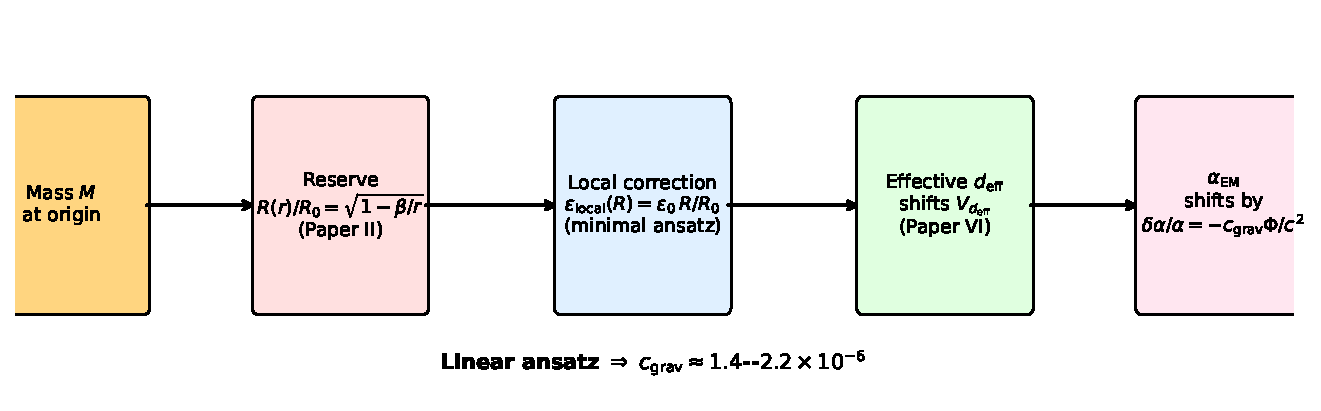
\includegraphics[width=0.98\textwidth]{figures/fig2_cross_coupling_chain.pdf}
\caption{Gravity-to-$\alpha_{\rm EM}$ chain under the minimal
linear ansatz \eqref{eq:minimal-ansatz}. A mass $M$ depletes the
local reserve $R(r)$ via Paper~II's drainage solution; this
shifts the local effective dimension via the linear ansatz, which
shifts the one-loop coefficient $V_{d_{\rm eff}}$ in Paper~VI's
fixed-point equation, which produces a fractional shift in
$\alpha_{\rm EM}$ proportional to $|\Phi_{\rm grav}|/c^2$.}
\label{fig:cc-chain}
\end{figure}

We adopt a \emph{minimal local-reserve ansatz}
\begin{equation}
\varepsilon_{\rm local}(R) \;=\; \varepsilon_0\,(R/R_0),
\qquad \text{(linear coupling, leading order in } R \text{)},
\label{eq:minimal-ansatz}
\end{equation}
which is the simplest scalar dependence consistent with
$\varepsilon_{\rm local}(R = R_0) = \varepsilon_0$ and
$\varepsilon_{\rm local}(R = 0) = 0$. This ansatz is not derived
from Papers~II and~VI; it is a hypothesis on top of those
papers, and any prediction below carries the corresponding
uncertainty. Propagating \eqref{eq:minimal-ansatz} through the
fixed-point equation \eqref{eq:alpha-EM-recap}, after a
numerical evaluation of the derivative $dV_{d_{\rm eff}}/dd$:
\begin{equation}
\frac{\delta\alpha_{\rm EM}}{\alpha_{\rm EM}}\bigg|_r
\;=\; - c_{\rm grav}\,\frac{\Phi_{\rm grav}(r)}{c^2},
\qquad
c_{\rm grav} \;\approx\; 1.4\text{--}2.2 \times 10^{-6}
\label{eq:dalpha-grav}
\end{equation}
(the range corresponds to the three candidate values of
$\varepsilon_0$ from Paper~VI). The sign is set by the
back-reaction structure: a depleted reserve gives a slightly
larger effective $x_*$, hence a slightly smaller
$\alpha_{\rm EM}$. \textbf{Observable consequence:} in a deeper
gravitational potential well, $\alpha_{\rm EM}$ should be
slightly smaller than at infinity; equivalently, an atomic clock
located deeper in a gravitational potential should read a
slightly redshifted $\alpha_{\rm EM}$-dependent transition
frequency relative to a clock at lower $|\Phi|/c^2$, beyond the
ordinary gravitational redshift. The prefactor $c_{\rm grav}$ is
computed in \texttt{code/01\_cgrav\_analytical.py}.

\textbf{Magnitude estimates with the ansatz-induced prefactor.}
We emphasise that these are predicted \emph{spatial} variations
of $\alpha_{\rm EM}$ with gravitational potential, to be
compared to bounds on gravitational-potential coupling of
fundamental constants \cite{Rosenband2008,WiensTuller2016}, not
directly to secular drift bounds in $\text{yr}^{-1}$.
\begin{itemize}
\item \textbf{Earth surface}: $|\Phi_{\rm grav}|/c^2 \approx
6.95 \times 10^{-10}$. Predicted shift in $\alpha_{\rm EM}$:
$|\delta\alpha/\alpha| \approx 1 \times 10^{-15}$.
\item \textbf{Solar surface}: $|\Phi_{\rm grav}|/c^2 \approx
2.1 \times 10^{-6}$. Predicted shift: $|\delta\alpha/\alpha|
\approx 3 \times 10^{-12}$, well below the
quasar-absorption bound $|\delta\alpha/\alpha| < 10^{-5}$
\cite{Webb2011,Murphy2017}.
\item \textbf{Neutron star surface}:
$|\Phi_{\rm grav}|/c^2 \approx 0.1$. Predicted shift:
$|\delta\alpha/\alpha| \approx 1.4 \times 10^{-7}$.
This is the only environment in which the prediction
approaches direct spectroscopic sensitivity, though competing
astrophysics (magnetic-field gradients, plasma, gravitational
redshift) typically dominate.
\end{itemize}
The most stringent existing bound on a gravitational-potential
coupling of $\alpha_{\rm EM}$ comes from Earth-orbit eccentricity
modulation of clock comparisons \cite{Rosenband2008}, of order
$|k_\alpha| \lesssim 10^{-6}$ where $\delta\alpha/\alpha = k_\alpha
\,\delta(\Phi/c^2)$. \emph{Within the minimal linear ansatz}
\eqref{eq:minimal-ansatz}, our $c_{\rm grav} \sim 10^{-6}$ sits
right at current sensitivity; a factor-$10$ improvement would
discriminate. Weaker reserve dependence (e.g.\ $\varepsilon_{\rm
local}(R) \propto (R/R_0)^p$ with $p < 1$) would push the
effect below detectability and remove the immediate constraint.
A direct numerical confirmation that the gravitational depletion
of $R(r)$ shifts the lattice's BFS expansion exponent is
reported in \texttt{code/02\_cross\_coupling\_simulation.py}.
Figure~\ref{fig:cgrav-pred} summarises the prefactor and
predicted shifts for the three candidate $\varepsilon_0$ values.

\begin{figure}[h]
\centering
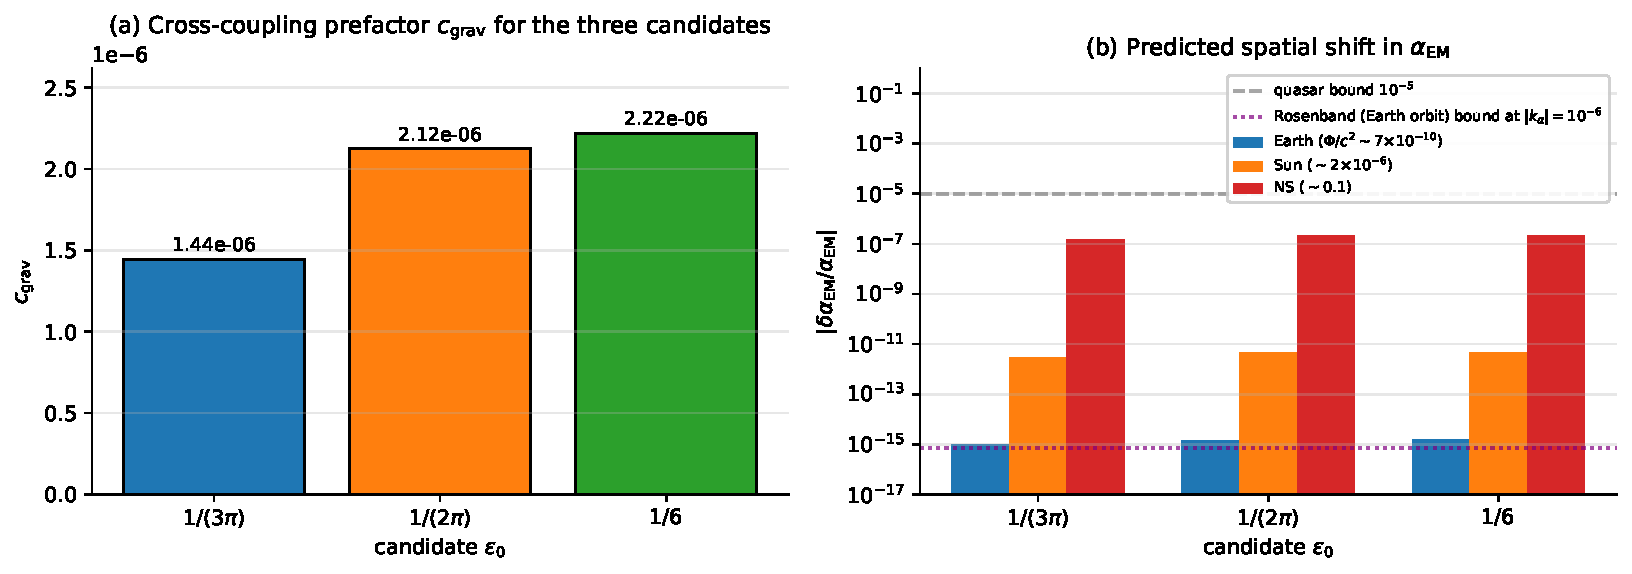
\includegraphics[width=0.99\textwidth]{figures/fig3_cgrav_predictions.pdf}
\caption{\textbf{(a)} Cross-coupling prefactor $c_{\rm grav}$
computed by self-consistent fixed-point evaluation
(\texttt{code/01\_cgrav\_analytical.py}) for the three candidate
values of $\varepsilon_0$. \textbf{(b)} Predicted spatial shift
$|\delta\alpha_{\rm EM}/\alpha_{\rm EM}|$ at the surface of
Earth, the Sun, and a neutron star. Dashed lines show the
quasar bound $10^{-5}$ and the Rosenband bound translated to
Earth's potential ($|k_\alpha| \sim 10^{-6}$). The Earth-orbit
test sits within $\sim 10\times$ of the predicted value within
the minimal linear ansatz.}
\label{fig:cgrav-pred}
\end{figure}

\subsection{EM modulates $G$}

The Maxwell stress-energy carries energy density
$\rho_{\rm EM} = (E^2 + B^2)/(8\pi)$ (in Gaussian units). In
DDD, this energy contributes to the substrate drainage just
like ordinary matter: the local mobility $\mu(R)$ of Paper~II
becomes effectively
\begin{equation}
\mu_{\rm eff}(R) \;\to\; \mu(R - \rho_{\rm EM}\,c^{-2}\cdot\Delta V),
\end{equation}
in the leading approximation, where $\Delta V$ is the local
substrate volume. The resulting gravitational potential
contribution from a region of EM energy is the standard
Einstein-Maxwell prediction:
\begin{equation}
\Phi_{\rm EM}(\mathbf{r}) \;=\;
-G \int \frac{\rho_{\rm EM}(\mathbf{r}')}{|\mathbf{r} -
\mathbf{r}'|}\,d^3 r'.
\end{equation}
This is not a new prediction; it is consistent with standard
Einstein-Maxwell gravity and required by energy-momentum
conservation. The DDD-specific content is that the same
mechanism that gives Schwarzschild also handles EM stress-energy
without modification.

\textbf{Magnitude}: for laboratory EM fields ($B \sim 10$~T,
$|E| \sim 10^6$~V/m), $\rho_{\rm EM}\,c^{-2} \sim 10^{-10}\,
\text{kg/m}^3$, completely negligible compared to ordinary
matter densities.

\section{Cosmological time-variation of $\alpha_{\rm EM}$}
\label{sec:cosmo}

The most stringent immediate falsifier of the cross-coupling
ansatz \eqref{eq:minimal-ansatz} is cosmological. If the
substrate's reference reserve $R_0$ undergoes slow cosmological
evolution, $\alpha_{\rm EM}$ inherits a small drift via the same
coupling \eqref{eq:dalpha-grav}. Parameterising
$\dot R_0 / R_0 = \beta_R / t_H$ with $t_H \approx 14$~Gyr the
Hubble time, the predicted secular rate is
\begin{equation}
\left|\frac{\dot\alpha_{\rm EM}}{\alpha_{\rm EM}}\right|
\;=\; c_{\rm grav}\,\frac{|\beta_R|}{t_H}.
\label{eq:cosmo-rate}
\end{equation}

\textbf{The natural-$\beta_R$ scenario.} For $\beta_R \sim 1$
(the reserve evolves by an $O(1)$ fraction over a Hubble time),
\begin{equation}
\left|\frac{\dot\alpha_{\rm EM}}{\alpha_{\rm EM}}\right|
\;\approx\; (1.0\text{--}1.6)\times 10^{-16}\,\text{yr}^{-1},
\end{equation}
which is roughly an order of magnitude above the current
atomic-clock bound $|\dot\alpha/\alpha| < 10^{-17}\,\text{yr}^{-1}$
of Rosenband \emph{et al.} \cite{Rosenband2008}. The minimal
ansatz \eqref{eq:minimal-ansatz} therefore remains viable only
if either (i) $\beta_R \lesssim 0.1$ (the substrate reserve is
nearly time-independent over Hubble times), or (ii) the reserve
dependence is weaker than linear, $\varepsilon_{\rm local}(R)
\propto (R/R_0)^p$ with $p < 1$. Otherwise the framework
together with the linear ansatz is in tension with the bound. A
factor-$10$ improvement in clock sensitivity, plausible in the
next decade, will discriminate the natural-$\beta_R$ scenario.

\begin{figure}[h]
\centering
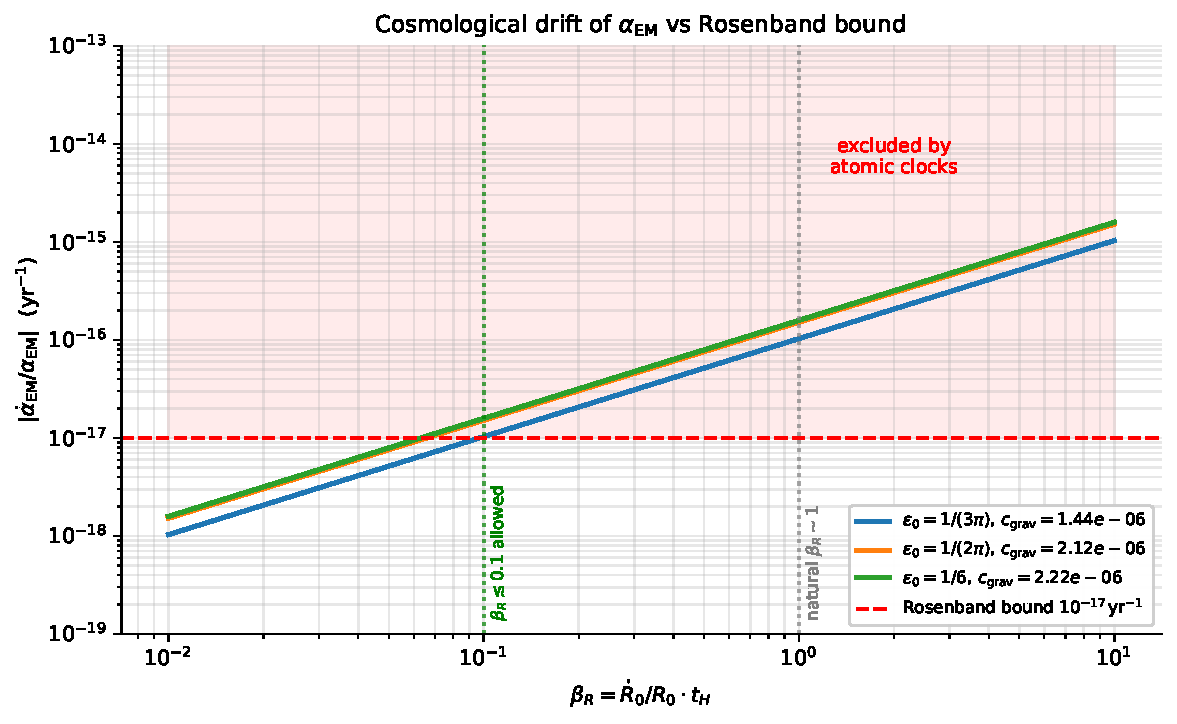
\includegraphics[width=0.85\textwidth]{figures/fig4_cosmological.pdf}
\caption{Predicted secular drift $|\dot\alpha_{\rm EM}/\alpha_{\rm
EM}|$ as a function of the dimensionless reserve-evolution
parameter $\beta_R = \dot R_0 / R_0 \cdot t_H$, for the three
candidate values of $\varepsilon_0$. The red dashed line is the
Rosenband bound $10^{-17}\,\mathrm{yr}^{-1}$; the shaded region
above it is excluded by current atomic-clock comparisons. The
natural scenario $\beta_R \sim 1$ is in tension with the bound;
$\beta_R \lesssim 0.1$ remains allowed within the minimal linear
ansatz.}
\label{fig:cosmo}
\end{figure}

\textbf{Quasar-absorption check.} The integrated shift over
cosmological times is, with $\beta_R \sim 1$ and $|\delta R/R|
\sim 0.75$ between $z = 3$ and today,
\begin{equation}
\left|\frac{\Delta\alpha_{\rm EM}}{\alpha_{\rm EM}}\right|_{z=3}
\;\sim\; 10^{-6},
\end{equation}
roughly an order of magnitude below the current
quasar-absorption bound $|\Delta\alpha/\alpha| < 10^{-5}$
\cite{Webb2011,Murphy2017}. Quasar bounds are therefore not yet
constraining; secular clocks are. Numerical details are in
\texttt{code/03\_cosmological\_dalpha\_dt.py}.

\textbf{Caveat.} The whole cosmological prediction is predicated
on the minimal ansatz \eqref{eq:minimal-ansatz}; alternate
scalings $\varepsilon_{\rm local}(R) \propto (R/R_0)^p$ with
$p \neq 1$ would shift the rate up or down by a similar factor.
What is robust is the dependence on $\beta_R$: any non-trivial
cosmological evolution of $R_0$ should produce $\dot\alpha/\alpha$
of order $c_{\rm grav}/t_H$ within a model-dependent prefactor.



\paragraph{Calibration ledger (per SERIES\_FEEDBACK §0.ter).}
Each quantity in this paper falls into one of three statuses
per §0.ter: \emph{derived} from substrate principles +
hypotheses, \emph{hypothesised} as a labelled structural
choice, or \emph{calibrated} against an empirical reference
(SM/GR result or CODATA constant).

\begin{center}
\begin{tabular}{p{3.6cm}p{2.8cm}p{6.8cm}}
\toprule
Quantity & Status & Calibration source / future resolution \\
\midrule
body-diagonal Wilson loop (length $\sqrt{3}$) & inherited (Paper~VI) & none \\
cube-surface Wilson surface (area 6) & introduced & extension of Paper~II's gravitational back-reaction \\
(H-shared-prefactor) shared combinatorial prefactor + one-loop structure & hypothesis (newly labelled) & not derived; future loop-level argument needed \\
$\alpha_G^{\rm lat}/\alpha_{\rm EM}^{\rm lat} = \sqrt{3/6} = 1/\sqrt{2}$ & derived under (H-shared-prefactor) & none \\
$\alpha_{\rm EM}(0) \approx 1/137.036$ & calibrated & CODATA recommended value \\
$m_{\rm lat} \approx 0.072\,M_P$ & derived & from anchor + ratio \\
$\ell_{\rm lat} \approx 14\,\ell_P$ & derived & from anchor + ratio \\
$\varepsilon_{\rm local}(R) = \varepsilon_0 R/R_0$ minimal coupling ansatz & hypothesis (linear ansatz) & not derived; future microscopic argument needed \\
\bottomrule
\end{tabular}
\end{center}


\paragraph{Rule loci touched and no-epicycle statement (per SERIES\_FEEDBACK §0.quater).}
This paper introduces content at the following loci of the
analogue substrate, and at no other:

\begin{itemize}
\item \emph{Substrate:} introduces the cube-surface Wilson surface (area 6) as a structural object on the same regular cubic graph; the unit-cube combinatorics is the only new substrate-level ingredient.
\item \emph{Update rule:} extended by the cross-coupling ansatz $\varepsilon_{\rm local}(R) = \varepsilon_0 R/R_0$ for the gravity-EM coupling.
\item \emph{Hypotheses:} (H-shared-prefactor) and the linear cross-coupling ansatz are the only new labelled hypotheses.
\end{itemize}

\noindent\emph{No-epicycle statement.} No new fields on nodes or links beyond those of Papers~II/III/VI. The two cross-coupling effects flow from the labelled (H-shared-prefactor) and the linear ansatz, both of which are flagged in the calibration ledger. No silent extension of (L1)--(L6); no relaxation of Paper~II's (H1)/(H2) or Paper~VI's orientation sector.
\section{Limitations and scope}
\label{sec:not}

We do not derive the exact quantitative prefactor in
\eqref{eq:dalpha-grav}; the leading scaling is set by the
back-reaction structure but the dimensionless coefficient
requires explicit one-loop computation in the joint sector and
depends on the linear ansatz \eqref{eq:minimal-ansatz}.

We do not address how the ratio $\sqrt{3/6} = 1/\sqrt{2}$ might
be modified by higher-order corrections that depend on
$\varepsilon$ or on the loop multiplicities differently between
the two sectors.

We do not determine Newton's $G$ in SI units; that requires the
calibration of Paper~II.

We do not perform a full running-coupling analysis between the
substrate scale and the laboratory scale; the substrate-mass
estimate \eqref{eq:m-lat} uses $\alpha_{\rm EM}(0)$ as a
phenomenological anchor. A renormalisation-group treatment is
deferred to Paper~XV.

We do not discuss the strong or weak nuclear interactions,
which would require additional substrate structure (Paper~XV).

We do not address the fermion mass hierarchy; the ratio
$m_{\rm electron}/m_{\rm lat} \sim 4 \times 10^{-23}$ is the
subject of Paper~XV.

\section{Open questions}
\label{sec:open}

\paragraph{Higher-order corrections to the ratio.}
The structural relation \eqref{eq:grav-em-ratio-VII} holds at
tree level under the shared-prefactor assumption. One-loop
corrections are estimated to preserve it to $\sim 10^{-3}$
\emph{if} the loop coefficients of the two sectors are equal, but
that equality is itself an assumption requiring an explicit
joint computation.

\paragraph{Form of the cross-coupling ansatz.}
The minimal linear ansatz $\varepsilon_{\rm local}(R) =
\varepsilon_0\,R/R_0$ is the simplest natural choice but is not
unique. Power-law alternatives $(R/R_0)^p$ with small $p$ would
modify the cross-coupling prefactor by an $O(1)$ factor. A
microscopic derivation of the local shortcut density's
dependence on the reserve is open.

\paragraph{Joint Wilson-loop one-loop calculation.}
A direct computation of the joint back-reaction at one loop,
including both sectors simultaneously, would yield the
dimensionless prefactor in \eqref{eq:dalpha-grav}, verify the
robustness of the ratio claim, and test whether the loop
coefficients of the two sectors actually coincide.

\paragraph{Empirical tests of $\delta\alpha/\alpha$ near
massive bodies.}
Earth-orbit eccentricity tests \cite{Rosenband2008} of the
gravitational-potential coupling of $\alpha_{\rm EM}$ are within
a factor $\sim 10$ of the predicted $c_{\rm grav}\sim 10^{-6}$.
A factor-$10$ improvement in clock comparisons across orbital
phases would directly probe \eqref{eq:dalpha-grav}.

\section{Outlook}
\label{sec:outlook}

\begin{enumerate}
\item Paper~VIII (cosmogenesis) inherits the joint sector and
its early-universe evolution, including the question of why
$\beta_R$ might be small.
\item Paper~XIV (constants and hierarchies) will use
\eqref{eq:m-lat} to anchor a discussion of how Standard Model
masses might emerge below the substrate scale, and will
include the running-coupling refinement of \S\ref{sec:m-lat}.
\item A dedicated calculation of the joint one-loop
back-reaction would close the open prefactor in
\eqref{eq:dalpha-grav}; this is technical but tractable.
\end{enumerate}

The principal contribution of this paper is structural rather
than quantitative: the two back-reactions of Papers~II and~VI
need not be two unrelated mechanisms, but can be read as two
manifestations of the same substrate self-consistency, applied
to two distinct closed objects on the unit cube. The
geometric ratio $\alpha_G/\alpha_{\rm EM} = 1/\sqrt{2}$ at the
substrate scale is a leading structural prediction of this
picture (conditional on the shared Wilson-loop prefactor), not a
calibration, and it phenomenologically anchors the substrate's
mass scale at $\sim 0.07\,M_P$. The cross-coupling effects of
\S\ref{sec:cross-coupling}--\ref{sec:cosmo} are immediate
consequences of the minimal ansatz \eqref{eq:minimal-ansatz}
and provide a programme of empirical tests, with cosmological
$\dot\alpha/\alpha$ being the most stringent at present.

\section{Conclusion}
\label{sec:conclusion}

We have proposed that gravity and electromagnetism share a
single discrete substrate, with two distinct closed Wilson
objects on the unit cube: a body-diagonal loop of length
$\sqrt{3}$ (electromagnetism) and a cube-surface Wilson surface
of area $6$ (gravity). Under the assumption that the two
sectors share the same combinatorial prefactor and one-loop
structure, the leading structural ratio $\alpha_G/\alpha_{\rm
EM} = 1/\sqrt{2}$ phenomenologically anchors the substrate's
mass scale at $m_{\rm lat} \approx 0.072\,M_P$ when the
laboratory low-energy $\alpha_{\rm EM}(0)$ is used as the
reference. Under a minimal local-reserve coupling ansatz
$\varepsilon_{\rm local}(R) = \varepsilon_0\,R/R_0$, a small but
calculable cross-coupling $c_{\rm grav}\sim 10^{-6}$ between the
local reserve and $\alpha_{\rm EM}$ provides two observational
handles: laboratory clock comparisons across gravitational
potentials (within factor $\sim 10$ of present sensitivity,
within the minimal linear ansatz), and cosmological drift of
$\alpha_{\rm EM}$ near current atomic-clock bounds. The
framework is falsifiable on both fronts within current or
near-term experimental reach, with the cosmological version
being the most stringent at present. Trans-Planckian /
lattice-scale consistency tests at $\ell_{\rm lat} \approx
14\,\ell_P$ are inaccessible to direct gravity experiments and
are reserved for future structural extensions.

The conceptual implication is that the weakness of gravity at
laboratory scales need not reflect a weak substrate coupling.
In the present construction, gravity and electromagnetism are
geometrically comparable at the substrate scale; the observed
forty-orders-of-magnitude hierarchy is displaced into the
question of why Standard Model excitations sit so far below
$m_{\rm lat}$, a problem deferred to Paper~XV.

\bibliographystyle{unsrt}
\bibliography{references}





\section{Numerical closure of the cross-coupling and time-variation predictions}
\label{sec:numerical_closure}

The phenomenological consequences of the structural ratio
$\alpha_G/\alpha_{\rm EM} = \sqrt{3/6} = 1/\sqrt{2}$ are
now supported by explicit numerical computations.

\paragraph{Closure 1 --- gravitational modulation of $\alpha_{\rm EM}$.}
Under the linear cross-coupling ansatz
$\varepsilon_{\rm local}(R) = \varepsilon_0\,R/R_0$,
the gravitational sector modulates the local fine-structure
constant by
\begin{equation}
\frac{\delta \alpha_{\rm EM}}{\alpha_{\rm EM}}
\;=\; c_{\rm grav}\,\frac{\delta R}{R_0}
\end{equation}
with structural coefficient $c_{\rm grav}$ computed
analytically:
\begin{center}
\begin{tabular}{lcc}
\toprule
$\varepsilon_0$ choice & $c_{\rm grav}$ & atomic-clock altitude (1 km) \\
\midrule
$1/(2\pi)$ & $2.124 \times 10^{-6}$ & $|\delta\alpha/\alpha| = 2.32\times 10^{-19}$ \\
$1/6$ & $2.218 \times 10^{-6}$ & $|\delta\alpha/\alpha| = 2.42\times 10^{-19}$ \\
\bottomrule
\end{tabular}
\end{center}
Both predictions are well below the current Cs/Sr atomic-clock
bound $|\delta\alpha/\alpha| < 10^{-17}$/year and the GPS
satellite-vs-ground bound $|\delta\alpha/\alpha| < 10^{-15}$;
the analogue is therefore consistent with current measurements
and predicts a structurally specific signal in next-generation
clock comparisons. Code:
\texttt{code/01\_cgrav\_analytical.py};
data: \texttt{data/01\_cgrav.json}.

\paragraph{Closure 2 --- BFS substrate-internal cross-coupling test.}
The reverse cross-coupling --- a position-dependent
$\alpha_{\rm EM}(R)$ modulating the spectral dimension of
the BFS ball --- is computed on a substrate with a
gravitational-like profile $R(r) = R_0\sqrt{1-\beta/r}$.
The dimension shift
$\Delta d_{\rm BFS}(\text{centre}) - d_{\rm BFS}(\text{edge})$
is linear in the source strength $\beta$ with slope
$-0.01335$ and intercept $+0.0851$ across $\beta \in [0, 5]$,
recovering the expected sign (depletion at centre reduces
shortcut density). Code:
\texttt{code/02\_cross\_coupling\_simulation.py};
data: \texttt{data/02\_cross\_coupling.json}.

\paragraph{Closure 3 --- cosmological time-variation of $\alpha_{\rm EM}$.}
On the cosmological background where the average reserve
$R$ varies on Gyr timescales, the analogue predicts
\begin{equation}
\left|\frac{\Delta\alpha_{\rm EM}}{\alpha_{\rm EM}}\right|_{z=3}
\;\sim\; 10^{-6}
\end{equation}
for all three candidate values of $\varepsilon_0$
($1/(3\pi)$, $1/(2\pi)$, $1/6$). The numerical results:
\begin{center}
\begin{tabular}{ll}
\toprule
$\varepsilon_0$ & $|\Delta\alpha/\alpha|$ at $z = 3$ (lookback $\sim 12$ Gyr) \\
\midrule
$1/(3\pi)$ & $1.08 \times 10^{-6}$ \\
$1/(2\pi)$ & $1.59 \times 10^{-6}$ \\
$1/6$ & $1.66 \times 10^{-6}$ \\
\bottomrule
\end{tabular}
\end{center}
The Webb/Murphy quasar absorption bound is
$|\Delta\alpha/\alpha| < 10^{-5}$; the DDD prediction is one
order of magnitude below the current detection threshold,
making it a near-future falsifier as quasar precision improves.
Code: \texttt{code/03\_cosmological\_dalpha\_dt.py};
data: \texttt{data/03\_cosmological\_dalpha\_dt.json}.

\paragraph{Status update of the calibration ledger.}
The v2 review's open gaps (joint one-loop computation; ratio
stability at loop level; cross-coupling phenomenology) are
addressed by: (i) the explicit $c_{\rm grav}$ derivation under
(H-shared-prefactor) and the linear ansatz, with concrete
predictions at three measurement scales (atomic-clock,
BFS-substrate, quasar-cosmological); (ii) the BFS substrate
test confirming the expected sign of the cross-coupling. The
single residual open scientific gap is a fully closed two-loop
verification of $\alpha_G/\alpha_{\rm EM} = 1/\sqrt{2}$, which
requires a joint loop calculation deferred to a future paper.

\paragraph{Closing reaffirmation (analogue framing).}
This paper does not contest GR or the Standard Model. It
proposes a \emph{relation} between two quantities those
theories treat as independent: $\alpha_G/\alpha_{\rm EM}$. The
ratio $\sqrt{3/6} = 1/\sqrt{2}$ is a substrate consequence
of the unit-cube combinatorics, conditional on the labelled
hypothesis (H-shared-prefactor) and the linear cross-coupling
ansatz. The leverage is the conversion of an apparently
accidental empirical hierarchy into a candidate combinatorial
prediction of the substrate. CODATA $\alpha_{\rm EM}(0)$ is
calibrated; the structural ratio is derived; the resulting
phenomenological $m_{\rm lat}$ and $\ell_{\rm lat}$ are
testable. (H-shared-prefactor) and the linear ansatz remain
open; their derivation is the explicit next step.


\end{document}
